%%%%%%%%%%%%%%%%%%%%%%%%%%%%%%%%%%%%%%%%%%%%%%%%%%%%%%%%%%%%%%%%%%%%%%%
%%%%%%%%%%%%%%%%%%%%%%%%%%%%%%%%%%%%%%%%%%%%%%%%%%%%%%%%%%%%%%%%%%%%%%%
%%%%%                                                                 %
%%%%%     <file_name>.tex                                             %
%%%%%                                                                 %
%%%%% Author:      <author>                                           %
%%%%% Created:     <date>                                             %
%%%%% Description: <description>                                      %
%%%%%                                                                 %
%%%%%%%%%%%%%%%%%%%%%%%%%%%%%%%%%%%%%%%%%%%%%%%%%%%%%%%%%%%%%%%%%%%%%%%
%%%%%%%%%%%%%%%%%%%%%%%%%%%%%%%%%%%%%%%%%%%%%%%%%%%%%%%%%%%%%%%%%%%%%%%

\chapter{Hardware Architecture}
Describe the architecture and the architectural decisions you
took. Blockdiagrams, the description of control, data flow and
interfaces go in here. Note that the architecture you present here
usually is more general than what you actually implemented and can
even be in a parameterized form.

\begin{figure}[tb]
  \centering
  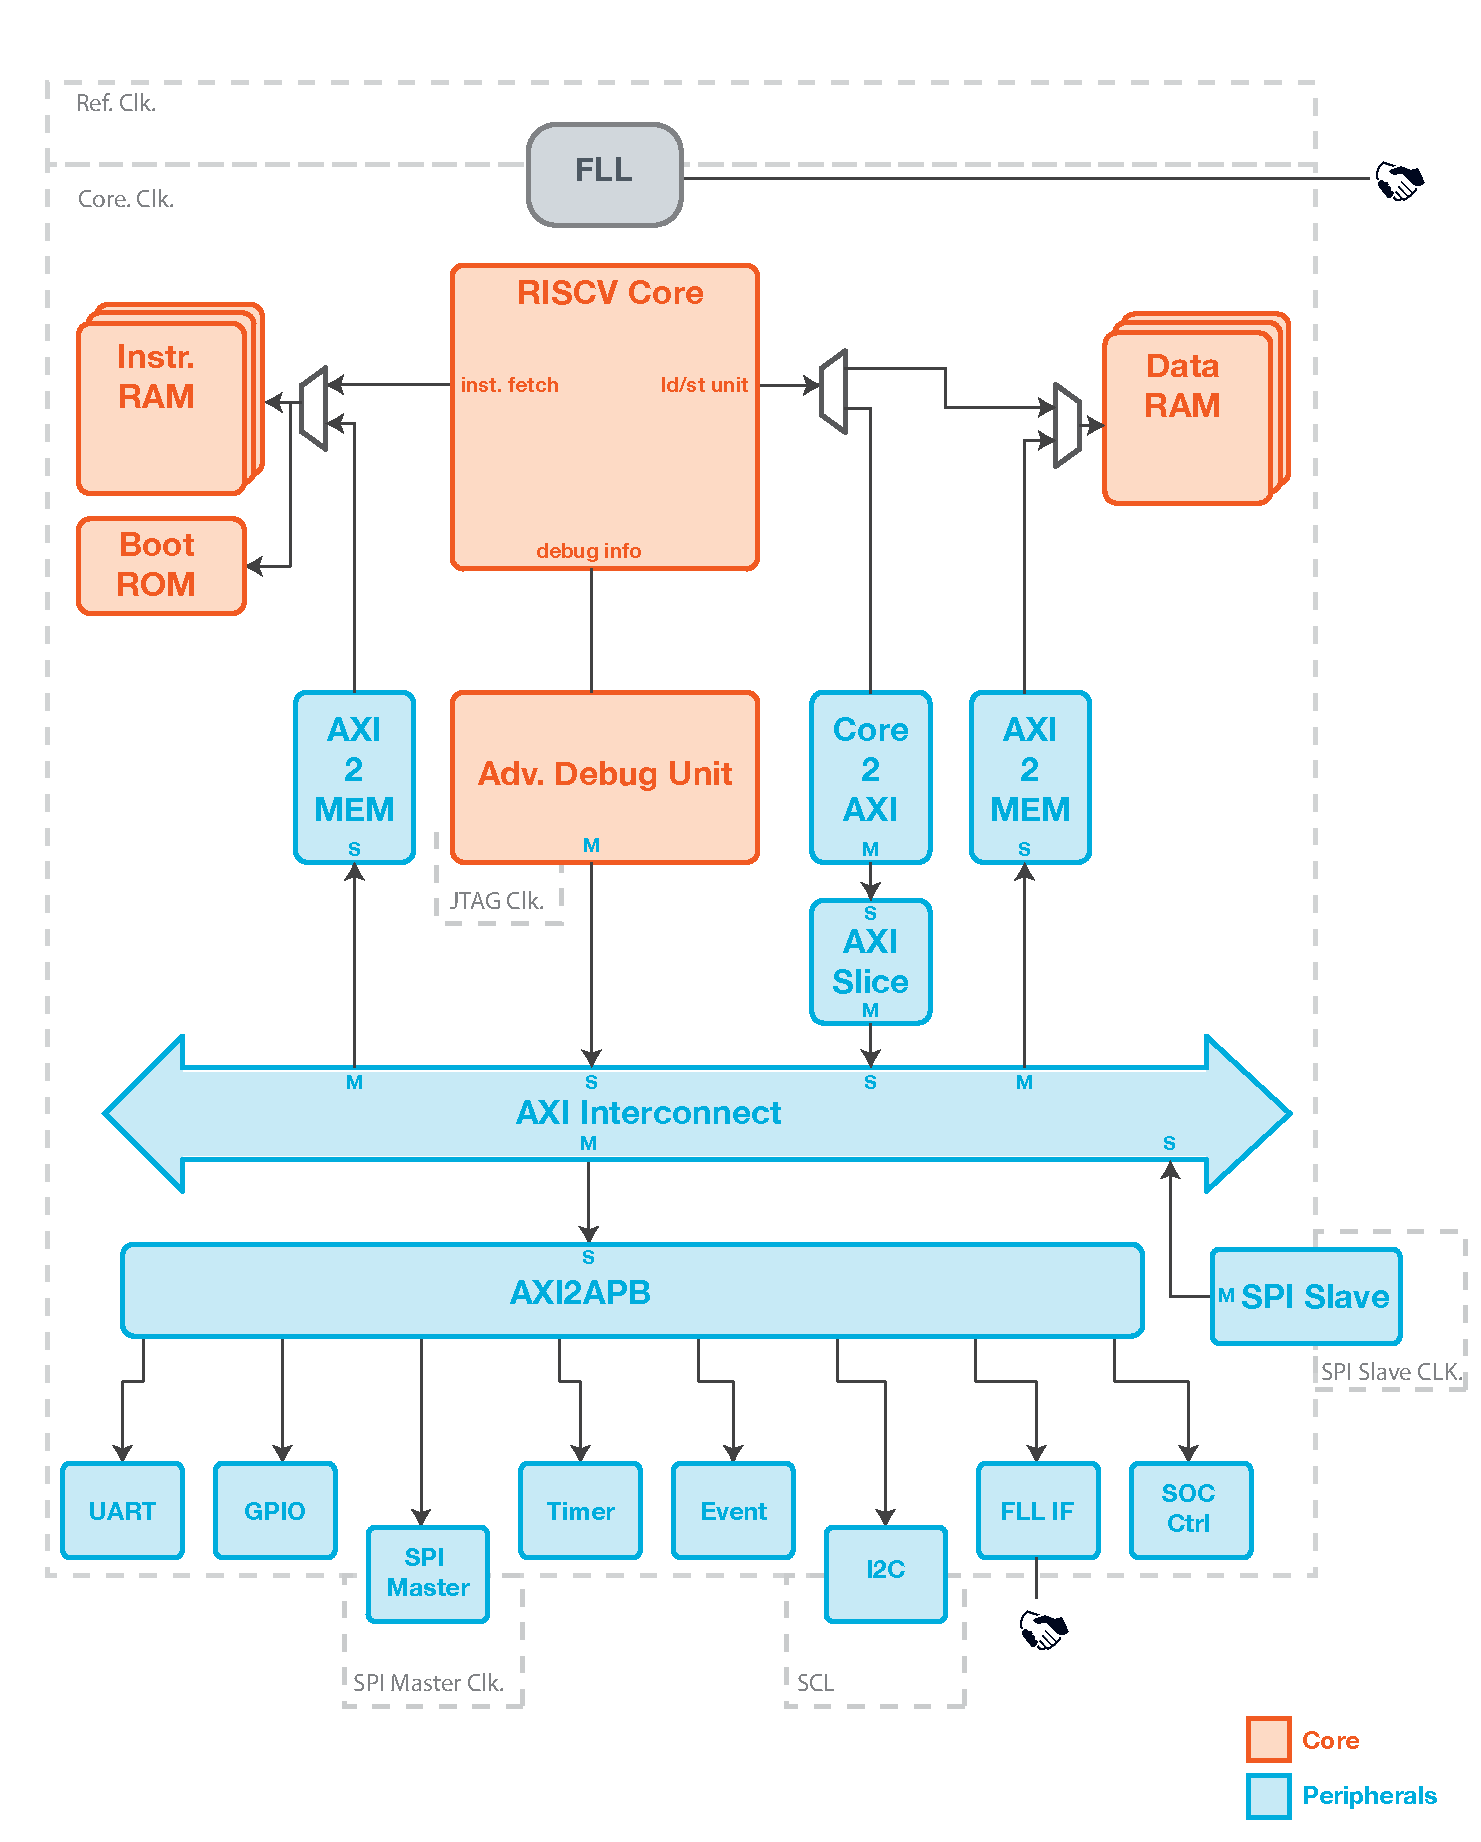
\includegraphics[width=\linewidth]{./figures/pulpino_blockdiagram}
  \caption{Functional verification setup.}
  \label{fig:block_diagram}
\end{figure}


\section{First Section}


\section{Second Section}
